\documentclass{article}

\usepackage[utf8]{inputenc}
\usepackage[a4paper]{geometry}
\usepackage{amsmath, amsfonts, amssymb, amsthm, mathtools}
\usepackage{graphicx}
\usepackage{parskip}
\usepackage{fancyhdr}
\usepackage{lastpage}
\usepackage{optidef}
\usepackage{hyperref}
\usepackage{tikz}

\usepackage[
style=authoryear]
{biblatex}
\addbibresource{sources.bib}

\pagestyle{fancy}
\fancyhf{}
\lhead{Ulrik Bernhardt Danielsen}
\rhead{Section \thesection}
\rfoot{Page \thepage \hspace{1pt} of \pageref{LastPage}}

\renewcommand{\headrulewidth}{1pt}
\renewcommand{\footrulewidth}{1pt}

\title{Specialization Project}
\author{Ulrik Bernhardt Danielsen}

\theoremstyle{plain}
\newtheorem{theorem}{Theorem}[section]
\newtheorem{lemma}{Lemma}[section]
\newtheorem{corollary}{Corollary}[theorem]
\newtheorem{proposition}{Proposition}[section]

\theoremstyle{definition}
\newtheorem{definition}{Definition}[section]
\newtheorem{example}{Example}[section]

\theoremstyle{remark}
\newtheorem*{remark}{Remark}

\begin{document}

\maketitle


\section{Task at hand}
Unsupervised clustering of behavioral patterns in rats based on 3D tracking of movements.
Tracking the rats posture has already been proven successful.
My task is to understand this methodology and for my thesis extend it to data including the faces of the rats \textcolor{red}{mainly whiskers?}.


\section{First look at the methodology}
\cite{Mimica} presents the decoding of distinct actions in figure \ref{fig:methodology_mimica}.
Section A shows how separate rats were fitted with the probes in two different positions.
\textcolor{red}{Why these positions?} The leftmost figure in section B shows which movements were recorded as time series data.
It records six different movements of the head, neck and back, along with the speed of the rats.
Then the data is \textit{detrended} and \textit{decomposed} spectrally using a Morlet wavelet transform. 
\textcolor{red}{This is maybe where I should start, no idea whats what this means.
The figure shows this as two steps, while the text as one (detrended \textit{using} Morlet).}
The next steps is reducing the dimensionality of the data \textcolor{red}{(wavelets?)}.  
This is done by finding the principal components explaining at least 95\% of the variance, before reducing non-linearly into only two dimensions using t-SNE (t-Stochastic Neighbor Embedding).
Using watershed segmentation on this two-dimensional mapping the discernible actions are found—44 in total.
The final part of the figure, C, shows the decoding accuracy for individual actions across animals.
The decoding accuracy are shown individually for four different cortices. 
\textcolor{red}{This I don't understand.
What are cortices, and what is decoding accuracy?}


\begin{figure}[h]
        \centering
        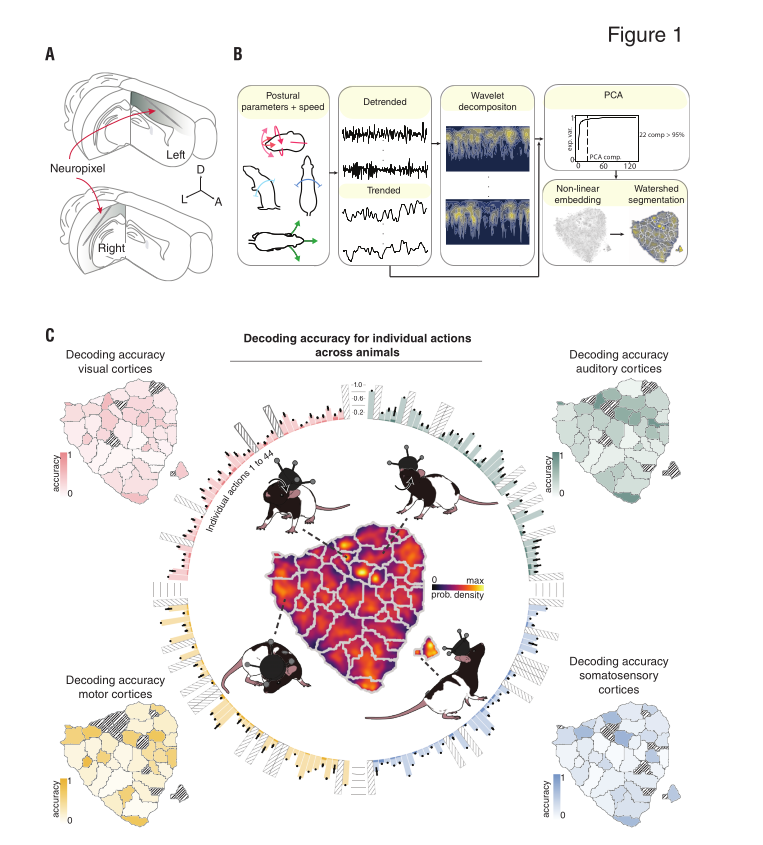
\includegraphics[width=0.6\linewidth]{./figures/methodology_mimica.png}
        \caption{Figure 1 in \cite{Mimica}.}
        \label{fig:methodology_mimica}
\end{figure}

\section{Berman paper}
The part which I will focus on is the methodology developed first in \cite{Berman}.
It develops a method for mapping distinct activities in fruit flies.
As stated there: \textit{The basis of our approach is to view behaviour as a trajectory through a high-dimensional space of postural dynamics.}

\subsection{Procedure}
\subsubsection{Postural decomposition}
Since they don't track the flies movements directly, and 40000 timeseries is a bit much, they first apply PCA to Radon transforms of the images.
They find that 50 postural modes are enough to explain a sufficient amount of variance.
\textcolor{red}{To do this they shuffle the dataset and compare the PCA eigenvalues of the data, to the largest one in a shuffled data set.
Is this also the procedure in our case?}
The individual movies can thus be transformed to a 50-dimensional timeseries, which they denote
\begin{equation*}
        \mathbf{Y} \equiv \{ y_1(t), y_2(t), \hdots , y_{50}(t) \}.
\end{equation*}
\textcolor{red}{This step does not seem to be of relevance to us.
I.e., no need to look up Radon transform?}

\subsection{Spectrogram generation}
First they state that looking for repeating sub-sequences in the time series are problematic, as \textit{certain behaviours involve multiple appendages moving at different time scales, this complicating the choice of motif length}.
Thus \cite{Berman} chooses another path—a \textit{spectrogram representation for the postural dynamics}.
The Morlet wavelet transform is supposed to be specially suited for dynamics over multiple time scales.
\textcolor{red}{They back this up by citing \textit{Daubechies I. 1992} Ten lectures on wavelets.
Might be a nice resource.}

\subsection{Spacial embedding}
The final step is to map the still very large feature vectors into a low dimensional (two-dimensional) space.
For this t-SNE is chosen.
Why?—because it does care much about preserving the "long" distances between the original features.
Many popular dimensionality reduction methods are tweaked for the opposite purpose, to keep the overall structure in mind.
\textcolor{red}{This argument should definitely be looked more into.}


\section{Steps:}
\begin{enumerate}
        \item z-scoring (standardization \textcolor{red}{although dividing by standard deviation is commented out})
        \item Smoothing by 3d splines
        \item Detrending around the smoothed curve \textcolor{red}{(Why do we need to do this? Do we expect trends?)}
        \item Morlet continuous wavelet transformation
                \begin{enumerate}
                        \item Hypothesis testing against 1st order autoregressive process
                        \item Smoothing of power across scales
                        \item Scale-averaged wavelet power
                        \item Rescaling features
                        \item Concatenating trend data and power spectrum
                \end{enumerate}
        \item PCA, reducing to feature dimension explaining at least 95\% of the variance
        \item t-SNE
        \item Watershed segmentation
\end{enumerate}
\newpage



\section{Introduction}
\subsection{Motivation}
The human brain is an incredibly complex structures that researchers have been trying to understand for a long time.
One way to gain information about how the brain operates is to study its neurons.
Neurons are cells which can communicate with each other through synapses.
This communication are electric signals and can be recorded.
\textcolor{red}{Source?}
At Kavli Institute for Systems Neuroscience at NTNU they are interested in relating these neural spike recordings to the behavior in rats.
This in turn begs the question of how rats behave.
Manually labelling video recordings of rats running around seems a tedious and unfruitful endeavor.
Additionally it introduces bias in our prior assumptions of how the rats behave, and which activities they engage in.
Thus, a methodology for automatically detecting distinct behaviours is needed.

\subsection{Previous work}
\textcolor{red}{Is this necessary?}


\section{Theory}
Concise description of the mathematical concepts used in the methodology.
\subsection{Time series}
\subsubsection{Detrending}
\subsubsection{Spectral analysis}
\subsubsection{Spline interpolation}
\subsubsection{Wavelet transformation}


\subsection{Dimensionality reduction}
\subsubsection{Principal Component Analysis}
\subsubsection{t-Stochastic Neighbor Embedding}

\subsection{Watershed segmentation}

\section{Methodology}
What is done in practice.
Discussion  of choices made.
\subsection{Input data}
\subsection{Feature extraction}
\subsection{Manifold embedding}








\newpage
\printbibliography
\end{document}



